Insbesondere aufgrund der immer größer werdenden Komplexität eingesetzter Technologien für den Softwareentwicklungs- und Deployment-Prozess, ist die Automatisierung im DevOps-Umfeld ein essentieller Bestandteil. Durch einen hohen Grad an Automatisierung sollen wiederholende Aufgaben reduziert werden, mit dem Ziel das Risiko manueller Fehler zu vermeiden und die Verschwendung von menschlichen Ressourcen zu minimieren. Gemäß des DevOps-Konzepts werden die Grundsätze des DevOps-Ansatzes durch den Aufbau einer Bereitstellungspipeline (engl. Deployment Pipeline) durchgesetzt. Die Deployment-Pipeline besteht im Wesentlichen aus mehreren Continuous Integration und Continuous Delivery-Pipelines und kann als eine automatisierte Implementierung der Build-, Test-, Deployment- und Release-Prozesse einer Anwendung definiert werden. \cite{humble_why_2011} Insbesondere die Testautomatisierung ist ein zentraler Bestandteil der Deployment Pipeline. Während zu Beginn einfache Unit-Tests ausreichen, müssen mit fortschreitender Automatisierung zur Sicherstellung der Qualität und Lauffähigkeit Funktions-, Last- oder Integrationstests implementiert werden, bis ein manuelles Testen bestenfalls überflüssig wird. \cite[S. 27]{alt_innovationsorientiertes_2017}, \cite[S. 110 - 111]{wolff_continuous_2016} Eine entsprechende Deployment-Pipeline kann durch den Einsatz passender Tools (dt. Werkzeuge)etabliert werden und stellt mit Hilfe miteinander kombinierter Tools eine optimale Abdeckung der Automatisierung sicher. \cite[S. 268]{tokarski_strategische_2018} Werden die Deployments automatisch in die Produktivumgebung ausgeführt, sind die DevOps-Teams ab diesem Zeitpunkt in der Lage, jederzeit eine neue Funktion, Fehlerbehebung oder Anpassungen an der Infrastruktur, auszuliefern. \cite{juner_praxisbasierte_2017} Wesentliche Ziele der Deployment-Pipeline sind, einen End-to-End-Prozess für alle sichtbar zu erstellen und durch die frühe Problemerkennung und -behebung das bestehende Feedback zu verbessern. \cite[S. 3 - 4]{humble_continuous_2011} In der Abbildung 8 wird die Deployment-Pipeline schemenhaft dargestellt und im Folgendem, anhand der Intergrations- und Delivery Pipeline näher erläutert.  

\begin{figure}[h]
    \centering
    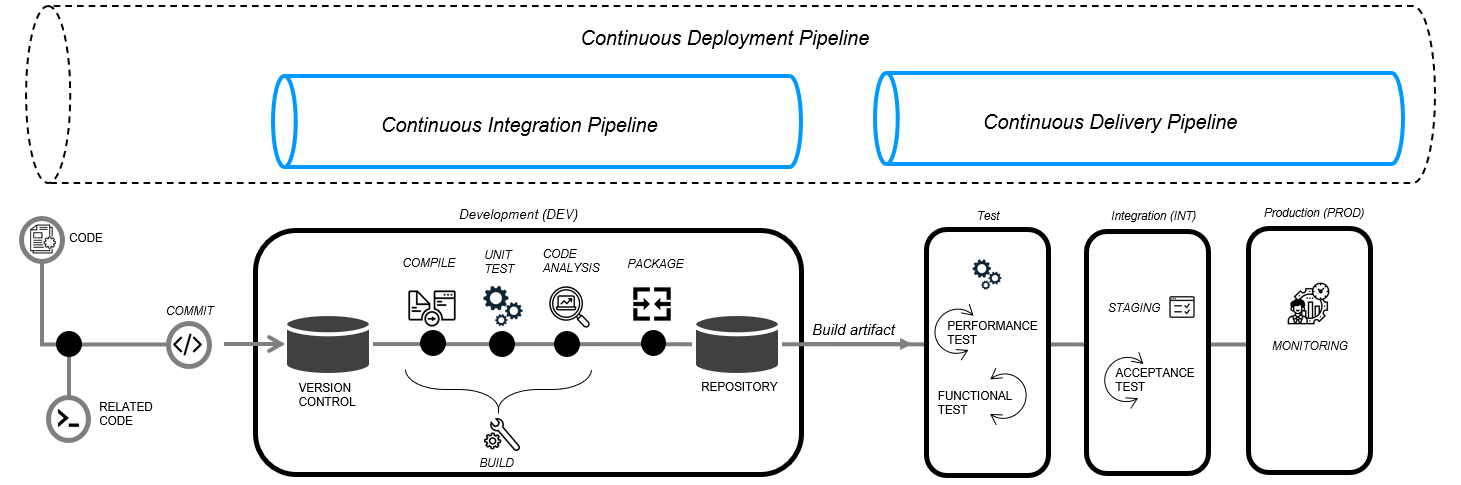
\includegraphics[scale=0.4]{Bilder/Continuous Deployment Pipeline.png}
    \caption{CD-Pipeline, angelehnt an \cite{balajee_what_2020}, \cite[S. 17]{sharma_devops_2017}}
\end{figure}

\paragraph{2.1.7.1. Integration Pipeline} $~$

Wie in der Abbildung 8 zu sehen ist, wird die Continuous Integration Pipeline zunächst bei jedem Einspielen von Code Commits automasiert angestoßen, wodurch der Code kompiliert wird und alle Unit-Tests durchgeführt werden. \cite[S. 266]{tokarski_strategische_2018}. Dabei erfolgen Unit-Tests automatisiert und ermöglichen ein schnelles Testen des Verhaltens von kleinen vorgenommenen Codeänderungen isoliert von den anderen Komponenten der Software. \cite[S. 60]{humble_continuous_2011} Nachdem das Testen erfolgreich abgeschlossen wurde, wird der Commit angenommen und die statische Analyse des Quellcodes kann beginnen. \cite[S. 61]{verona_practical_2016} Diese liefert Informationen über den Zustand des Codes, über Defekte, Design-Probleme oder ob Schwachstellen in den Bibliotheken von Drittanbietern gefunden wurden. \cite[S. 61]{verona_practical_2016}\\\\ Wichtige Voraussetzung für die Integration der CI-Pipeline ist zunächst die Verwendung einer Versionskontrolle. \cite[S. 100 - 101]{bass_devops_2015}, \cite[S. 57]{forsgren_mindset_2019} Diese ermöglicht es einzelnen Entwicklern, unabhängig von ihrem Standort oder von der Funktion, an der sie arbeiten, parallel zusammenzuarbeiten und sofort kleine Änderungen an dem Code zu erfassen. \cite[S. 57]{humble_continuous_2011} Um automatische Tests und Zusammenspiel aller Funktionen auf dem integrierten Master-Branch sicherzustellen und zeitaufwendige Code-Merges zu vermeiden, müssen insbesondere Feature-Branches bei der Entwicklung kurz gehalten werden. \cite{meyer_continuous_2014} Folglich soll die gesamte Entwicklung der Features in einem Branch in der Versionskontrolle und nicht auf dem Master-Branch stattfinden, wodurch die Entwickler an einem bestimmten Feature arbeiten können, ohne die Codebasis innerhalb des Master-Branches zu behindern. \cite[S. 44 - 45]{verona_practical_2016} Sobald Änderungen mit dem Main-Branch zusammengeführt werden, werden diese in automatischen Build-Prozessen und mittels Tests validiert. Nach der Validierung des Quellcodes wird dieser innerhalb eines Intergrationsservers (CI-Server) als ein Build erstellt in einem Repository veröffentlicht. Bei Änderungen des Builds werden erneut Unit-Tests durchgeführt, um die Funktionalität der Anpassung sicherzustellen. \cite[S. 57]{forsgren_mindset_2019} 


\paragraph{2.1.7.2. Delivery Pipeline} $~$

Die Continuous Delivery Pipeline erweitert die CI-Pipeline, um die erfolgreich durchgeführten Builds automatisch in produktionsähnlichen Testumgebungen bereitzustellen, in denen funktionale Test, Integrationstests und Performance-Tests durchgeführt werden. \cite[S. 17]{sharma_devops_2017} Wie in der Abbildung 8 dargestellt, ist der Auslöser für die CD-Pipeline jedes neue Build-Artefakt, welches im Repository veröffentlicht wird. Zusätzlich zum Quellcode werden alle Build-Artefakte innerhalb des Repositorys gespeichert, während die gleichen Versionen für die Entwicklungs-, Test- sowie Produktionsumgebung verwendet werden. \cite[S. 109 - 110]{kim_devops-handbuch_2017} Im nächsten Schritt wird der Code zusammen mit der entsprechenden Konfiguration, als ein Artefakt Build, also eine ausführbare Anwendung gebaut und sollte ab diesem Zeitpunkt nicht mehr verändert werden. In diesem Rahmen führt der CI-Server systemübergreifende Integrationstests an dem jeweiligen Build auf der Integrationsumgebung vor, um die fehlerfreie Interaktion der gesamten Komponenten miteinander zu testen. \cite[S. 122]{kim_devops-handbuch_2017} Während der Integrationstest wird eine Anbindung zu einer Testdatenbank konfiguriert, die aus einer ausreichenden Menge von Daten besteht, um die mit der Integration verbundenen automatisierten Tests durchzuführen. \cite[S. 100 - 101]{bass_devops_2015} Als nächsten Schritt wird die Software innerhalb der Staging-Umgebung, als eine produktionsähnliche Umgebung testweise betrieben, ohne die Interaktion der produktiv betriebenen Services. \cite[S. 100 - 101]{bass_devops_2015} Anschließend erfolgen die Akzeptanztests, die mit einer Anzahl von Nutzern festgelegte Use Cases der Anwendung testen und direktes Feedback über Schwachstellen oder funktionale Probleme liefern. \cite[S. 16 - 18]{sharma_devops_2017} Ferner können die Akzeptanztests auch automatisiert eingesetzt werden, was wiederrum den Grad der Wiederholbarkeit erhöht. Im Anschluss werden nicht-funktionale Tests und Performance-Tests durchgeführt.\\\\ Im besten Fall wird der Build durch die CD-Pipeline automatisch in die Produktivumgebung bereitgestellt, vorausgesetzt alle Tests wurden erfolgreich bestanden, anderenfalls wird das Deployment gestoppt und das Team wird über den Zustand des Builds informiert. \cite[S. 64]{forsgren_mindset_2019} Nachdem die Anwendung auf den normalen Produktivumgebung bereitgestellt wird, läuft diese konstant in einer Version oder aus einer Kombination von mehreren Versionen (Microservices). \cite[S. 86]{kim_devops-handbuch_2017} Die Architektur des Microservices bildet die Grundlage für den DevOps-Ansatz und beschreibt den Aufbau von Anwendungen, basierend auf eine große Anzahl an kleinen Services. \cite{sollner_devops_2017} Diese Services bestehen aus kleinen separaten funktionalen Codeteilen, die miteinander interagieren und miteinander ein Anwendungssystem abbilden. Oftmals wird nur eine Funktionalität abgebildet und kommuniziert mit anderen Services über eine definierte Schnittstelle. Mittels Microservices lassen sich einzelne Funktionalitäten leicht und schnell deployen und anpassen, wodurch das gesamte Deployment erhöht, die Wartung vereinfacht und das restliche System nicht gefährdet wird. \cite[S. 85 - 86]{kim_devops-handbuch_2017} Dieser Ansatz vereinfacht die Methode des Continuous Integration.

% Insgesamt lässt sich die Continuous Deployment Pipeline als einen automatischen, regelmäßigen Prozess der Bereitstellung erfolgreicher Builds in die Produktivumgebung beschreiben.

%Frage an Daniel: 
%1. Feature-Toggling, verschiedenes Testing (A/B-Tests, Canary-Tests, Live Test oder Beta-Tests), oder das Blue/Green Deployment erwähnen/beschreiben/erklären?????
%2. Irgeendwie bin ich mir nicht sicher, bei der Kapitelüberschrift---> Idee?



% Insbesondere die Testautomatisierung ist ein zentraler Bestandteil der Deployment Pipeline, da jede neue Version eines Builds über mehrere Schritte getestet, wiederholt getestet und anschließend an die Produktivumgebung übergeben werden muss.

% Um die Rolle der Automatisierung voranzutreiben, werden möglichst viele vollautomatisierte Deployments auf die Produktivumgebung aufgesetzt. 




 











  











 





